% Author: Seongjin Lee
% Hanyang University, Seoul, Korea
% esos.hanyang.ac.kr
% 2016-09-20
% note: some slides are adopted from  \url{www.cs.stevens.edu/~jschauma/631A/}
% https://github.com/resourceful/lecture_sysprog/

\documentclass[newPxFont,sthlmFooter,nooffset]{beamer}
\usepackage{kotex}
%\usetheme{sthlm}
\usepackage{../beamer_template/beamerthemesthlm}
\hypersetup{pdfauthor={Seongjin Lee (insight@gnu.ac.kr)},
            pdfsubject={Lecture Note: System Programming},
            pdfkeywords={Lecture Note, System Programming, class, (under)graduate},
            pdfmoddate={D: \pdfdate},
            pdfcreator={Seongjin Lee}}

%\setbeamertemplate{footline}[text line]{%
%    \parbox{\linewidth}{\vspace*{-8pt} \insertsectionhead  \hfill\insertshortauthor\hfill\insertpagenumber}}
%\setbeamertemplate{navigation symbols}{}




\title{System Programming}
\subtitle{Week 6: Process Control}
\author[SJL]{Seongjin Lee}
\institute{\href{mailto:insight@gnu.ac.kr}{insight@gnu.ac.kr}\\\url{http://open.gnu.ac.kr}\\Systems Research Lab.\\Gyeongsang National University}
\date{\today}

\begin{document}



\frame[plain]{\titlepage}

\frame{\frametitle{Table of contents}\tableofcontents}


%---------------------------------------------------------



\begin{frame}[t]
  \frametitle{introduction}
This chapter covers following items
  \begin{itemize}
  \item Creation of new processes, program execution, and process termination
  \item Properties of Process
  \item Interpreter files and the \texttt{system} function
  \item Miscellaneous
  \end{itemize}

\end{frame}


\begin{frame}[t]
  \frametitle{Process Identifiers}
Every process has a unique process ID (a non-negative integer)
\begin{itemize}
\item Although they are unique, the IDs are reused after termination
\item Process ID 0 is usually the scheduler known as the \textit{swapper}
\item Process ID 1 is usually the \texttt{init} process (invoked at the end of the boostrap procedure, located in \texttt{/etc/init} or \texttt{/sbin/init})
\item Process ID 2 is \textit{pagedaemon} responsible for supporting the paging of the virtual memory system
\end{itemize}
\end{frame}

\begin{frame}[containsverbatim,t]
  \frametitle{Functions to find the identifiers}
\begin{codedef}
#include <unistd.h>
pid_t getpid(void);
// Returns: process ID of calling process

pid_t getppid(void);
// Returns: parent process ID of calling process

uid_t getuid(void);
// Returns: real user ID of calling process

uid_t geteuid(void);
// Returns: effective user ID of calling process

gid_t getgid(void);
// Returns: real group ID of calling process

gid_t getegid(void);
// Returns: effective group ID of calling process
\end{codedef}
\end{frame}

\section{Process creation, execution, and termination}

\subsection{Process Creation}
\begin{frame}[containsverbatim,t]
  \frametitle{\texttt{fork(2)} Function}

The new process created by \texttt{fork} is called the \textit{child process}

\begin{codedef}
#include <unistd.h>
pid_t fork(void);
// Returns: 0 in child, process ID of child in parent, -1 on error
\end{codedef}
\end{frame}

\begin{frame}[t]
  \frametitle{\texttt{fork(2)} Function cont'd}
\texttt{fork} is called once but returns twice
\begin{itemize}
\item The return value in the child is 0
\item The return value in the parent is the process ID of the new child
\item The child is copy of the parent
\item Both the child and the parent continue executing with the instruction that follows the call to \texttt{fork}
\end{itemize}

Must understand that
\begin{itemize}
\item The order of execution of the child and the parent depends on the scheduling algorithm
\item The parent and the child share the same file offset
\item The child has its own copy of the parent's descriptors
\end{itemize}
\end{frame}


\begin{frame}[containsverbatim,t]
  \frametitle{\texttt{fork(2)} Example}
\lstinputlisting[linerange={7-23},lineskip=0em]{codes/fork.c}

\end{frame}


\begin{frame}[fragile,containsverbatim,t]
  \frametitle{\texttt{fork(2)} Example}

\begin{verbatim}
make fork
./fork
./fork | cat
\end{verbatim}

When we write to standard output
\begin{itemize}
\item we subtract 1 from the size of \texttt{buf} to avoid writing the terminating null byte
\item \texttt{strlen} calculate the length of a string not including the terminating null byte
  \begin{itemize}
  \item \footnotesize \texttt{strlen} requires function call
  \end{itemize}
\item \texttt{sizeof} calculate the length of string including the terminating null byte
  \begin{itemize}
  \item \footnotesize \texttt{sizeof} calculates the buffer length at compile time
  \end{itemize}
\end{itemize}

If buffer is not flushed before \texttt{fork}, the buffer is copied to child
\end{frame}

\begin{frame}
  \frametitle{Sharing of Open Files}
  \begin{figure}[h]
    \centering
    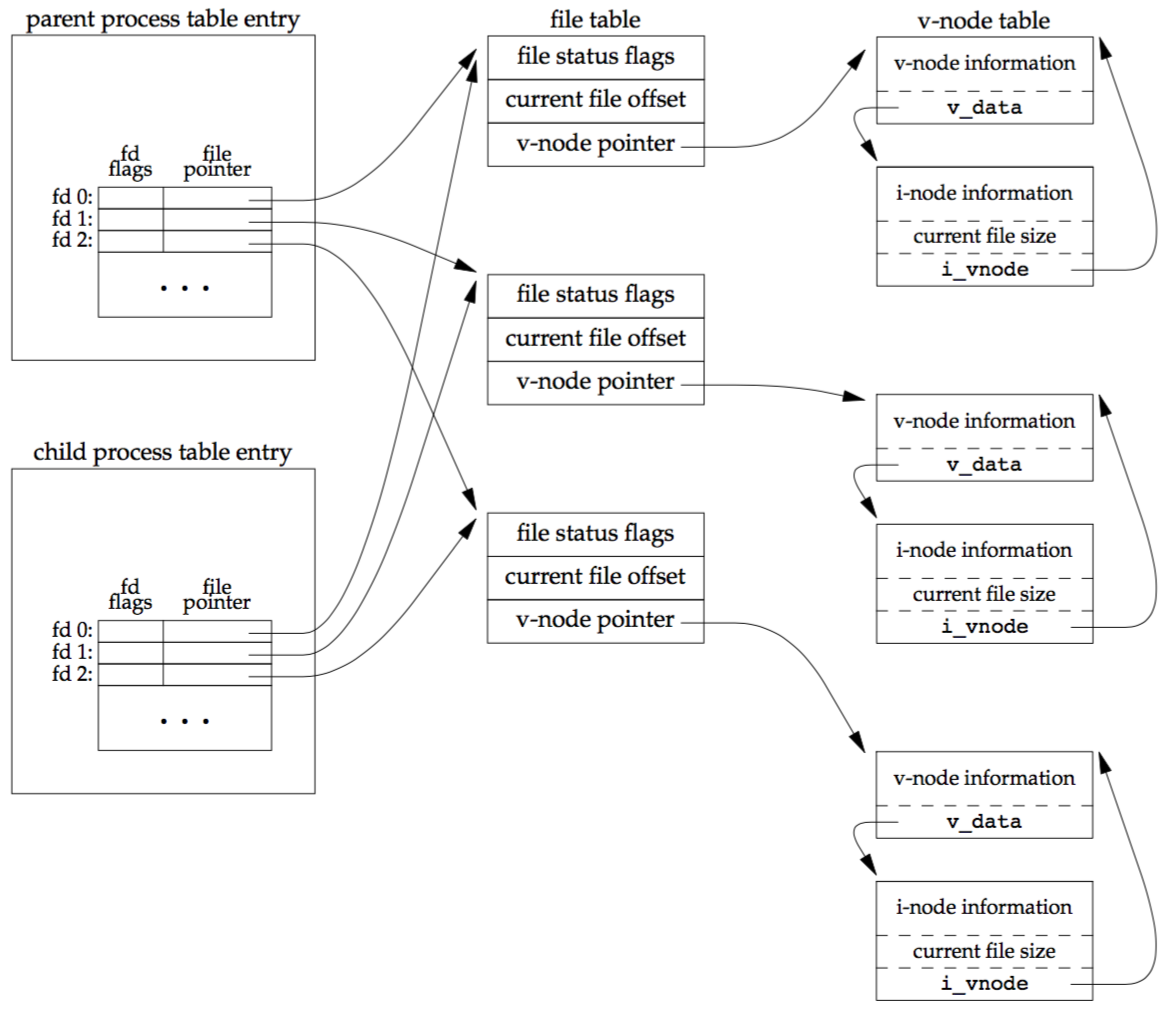
\includegraphics[height=0.9\textheight]{figure/fig8-2_sharing.png}
    \caption{Sharing of open files between parent and child after \texttt{fork}}
  \end{figure}
\end{frame}


\begin{frame}[t]
  \frametitle{Two normal cases for handling the descriptors after a
    \texttt{fork}}

the parent waits for the child to complete
\begin{itemize}
\item the parent does not need to do anything with its descriptors
\item when the child terminates, any of the shared descriptors that the child read from or wrote to will have their file offsets updated accordingly
\end{itemize}

Both the parent and the child go their own ways
\begin{itemize}
\item after the \texttt{fork}, the parent and the child closes the descriptors that it doesn't need
\end{itemize}
\end{frame}


\begin{frame}
  \frametitle{Properties that child inherits}
  \begin{itemize}
  \item  Real user ID, real group ID, effective user ID, and effective group ID
  \item  Supplementary group IDs
  \item  Process group ID
  \item  Session ID
  \item  Controlling terminal
  \item  The set-user-ID and set-group-ID flags
  \item  Current working directory
  \item  Root directory
  \item  File mode creation mask
  \item  Signal mask and dispositions
  \item  The close-on-exec flag for any open file descriptors
  \item  Environment
  \item  Attached shared memory segments
  \item  Memory mappings
  \item  Resource limits
  \end{itemize}
\end{frame}



\begin{comment}
  \begin{frame}
    \frametitle{The differences are}
    \begin{itemize}
    \item The return values from fork are different.
    \item The process IDs are different.
    \item The two processes have different parent process IDs: the
      parent process ID of the child is the parent; the parent process
      ID of the parent doesn’t change.
    \item The child's \texttt{tms\_utime}, \texttt{tms\_stime},
      \texttt{tms\_cutime}, and \texttt{tms\_cstime} values are set to
      0 (these times are discussed in Section 8.17).
    \item File locks set by the parent are not inherited by the child.
    \item Pending alarms are cleared for the child.
    \item The set of pending signals for the child is set to the empty
      set.
    \end{itemize}
  \end{frame}
\end{comment}


\begin{frame}[t]
  \frametitle{Why do \texttt{fork} fail}
  \begin{itemize}
  \item if too many processes are already in the system
  \item if the total number of processes for this real user ID exceeds the system's limit (\texttt{CHILD\_MAX})
  \end{itemize}
\end{frame}


\begin{frame}[t]
  \frametitle{Two uses for \texttt{fork}}
  \begin{itemize}
  \item  When a process wants to duplicate itself so that the parent and the child can each execute different sections of code at the same time.
    \begin{itemize}
    \item This is common for network servers.
    \end{itemize}
  \item When a process wants to execute a different program.
    \begin{itemize}
    \item This is common for shells. In this case, the child does an
      \texttt{exec} right after it returns from the fork.
    \end{itemize}

  \end{itemize}
\end{frame}


\subsection{Process Termination}
\begin{frame}[t]
  \frametitle{\texttt{exit} Functions}
Process can terminate normally in five ways
  \begin{itemize}
  \item Executing a return from the main function.
    % \begin{itemize}
    % \item \footnotesize This is equivalent to calling exit.
    % \end{itemize}

  \item Calling the exit function.
    % \begin{itemize}
    % \item \footnotesize This function is defined by ISO C and includes
    %   the calling of all exit handlers that have been registered by
    %   calling atexit and closing all standard I/O streams.
    % \end{itemize}

  \item Calling the \texttt{\_exit} or \texttt{\_Exit} function.
    % \begin{itemize}
    % \item \footnotesize ISO C defines \texttt{\_Exit} to provide a way
    %   for a process to terminate without running exit handlers or
    %   signal handlers.
    % \item \footnotesize Whether standard I/O streams are flushed
    %   depends on the implementation.
    % \item \footnotesize On UNIX systems, \texttt{\_Exit} and
    %   \texttt{\_exit} are synonymous and do not flush standard I/O
    %   streams.
    % \item \footnotesize The \texttt{\_exit} function is called by
    %   \texttt{exit} and handles the UNIX system-specific details;
    %   \texttt{\_exit} is specified by POSIX.1.
    % \item \footnotesize In most UNIX system implementations,
    %   \texttt{exit(3)} is a function in the standard C library,
    %   whereas \texttt{\_exit(2)} is a system call.
    % \end{itemize}

  \item Executing a return from the start routine of the last thread
    in the process.
    % \begin{itemize}
    % \item \footnotesize The return value of the thread is not used as
    %   the return value of the process. When the last thread returns
    %   from its start routine, the process exits with a termination
    %   status of 0.
    % \end{itemize}

  \item Calling the \texttt{pthread\_exit} function from the last
    thread in the process.
  \end{itemize}

Regardless of how a process terminates, the same code in the kernel is eventually executed
\begin{itemize}
\item the code closes all the open descriptors for the process
\item releases the memory that it was using
\end{itemize}
\end{frame}



\begin{frame}[t]
  \frametitle{\texttt{wait(2)} \texttt{waitpid(2)} Function}
When a process terminates, either normally or abnormally, the kernel notifies the parent by sending the \texttt{SIGCHLD} signal to the parent
\begin{itemize}
\item This signal is asynchronous notification from the kernel to the parent
\item parent can choose to ignore this signal
\item parent can provide a function (signal handler) that is called when the signal occurs
\end{itemize}

A process that calls \texttt{wait} or \texttt{waitpid} can
\begin{itemize}
\item block, if all of its children are still running
\item return immediately with the termination status of a child, if a child has terminated and is waiting for its termination status to be fetched
\item return immediately with an error, if it doesn't have any child processes
\end{itemize}
\end{frame}

\begin{frame}[containsverbatim,t]
  \frametitle{\texttt{wait(2)} \texttt{waitpid(2)} Function}

\begin{codedef}
#include <sys/wait.h>
pid_t wait(int *statloc);
pid_t waitpid(pid_t pid, int *statloc, int options);
// Both return: process ID if OK, 0 (see later), or -1 on error
\end{codedef}

\begin{itemize}
\item The \texttt{wait} function can block the caller until a child process terminates, whereas \texttt{waitpid} has an option that prevents it from blocking
\item The \texttt{waitpid} function doesn't wait for the child that terminates first; it has number of options that control which process it waits for
\end{itemize}

\texttt{statloc} is a pointer to an integer
\begin{itemize}
\item if this is not a null pointer, the termination status of the terminated process is stored in the location pointed to by the argument
\end{itemize}
\end{frame}

\begin{frame}[containsverbatim,t]
  \frametitle{\texttt{wait(2)} \texttt{waitpid(2)} Function}
if we have more than one child, wait returns on termination of any of the children

we need is a function that waits for a specific process: \texttt{waitpid}
The interpretation of the pid argument for waitpid depends on its value:
\begin{description}
\item [\texttt{pid == -1}] waits for any child process, \texttt{waitpid} is equivalent to \texttt{wait}
\item [\texttt{pid>0}] waits for the child whose process ID equals \textit{pid}
\item[\texttt{pid == 0}] waits for any child whose process group ID equals that of the calling process
\item[\texttt{pid < -1}] waits for any child whose process group ID equals the absolute value of pid
\end{description}

The waitpid function returns the process ID of the child that terminated and stores the child’s termination status in the memory location pointed to by statloc
\end{frame}


\begin{frame}[t]
  \frametitle{Macros to examine the termination status}
If we get the termination status in \texttt{status}, we can determine how a child died
\begin{description}
\item[\texttt{WIFEXITED(status)}] true if the child terminated normally
  \begin{itemize}
  \item \footnotesize we can execute \texttt{WEXITSTATUS(status)} to fetch the status
  \end{itemize}
\item[\texttt{WIFSIGNALED(status)}] true if status was child terminated abnormally that it didn't catch
  \begin{itemize}
  \item \footnotesize \texttt{WTERMSIG(status)} to fetch signal number that caused the termination
  \item \footnotesize \texttt{WCOREDUMP(status)} that returns true if a core file or the terminated process was generated
  \end{itemize}
\item[\texttt{WIFSTOPPED(status)}] true if status was returned for a child that is currently stopped
  \begin{itemize}
  \item \footnotesize \texttt{WSTOPSIG(status)} to fetch the signal number that caused the child to stop
  \end{itemize}
\item[\texttt{WIFCONTINUED(status)}] true if status was returned for a child that has been continued after a job control stop
\end{description}
\end{frame}

\begin{frame}[containsverbatim,t]
  \frametitle{\texttt{wait(2)} \texttt{waitpid(2)} Function}
The options argument lets us further control the operation of waitpid. This argument either is 0 or is constructed from the bitwise OR of the constants
  \begin{description}
  \item[\texttt{WCONTINUED}] If the implementation supports job
    control, the status of any child specified by \textit{pid} that
    has been continued after being stopped, but whose status has not
    yet been reported, is returned
  \item[\texttt{WNOHANG}] The \texttt{waitpid} function will not block
    if a child specified by pid is not immediately available. In this
    case, the return value is 0
  \item[\texttt{WUNTRACED}] If the implementation supports job
    control, the status of any child specified by \textit{pid} that
    has stopped, and whose status has not been reported since it has
    stopped, is returned. The \texttt{WIFSTOPPED} macro determines
    whether the return value corresponds to a stopped child process
  \end{description}
\end{frame}


\begin{frame}[t]
  \frametitle{three features of \texttt{waitpid} functions }
  \begin{itemize}
  \item The \texttt{waitpid} function lets us wait for one particular
    process, whereas the wait function returns the status of any
    terminated child.
  \item The \texttt{waitpid} function provides a nonblocking version
    of wait. There are times when we want to fetch a child’s status,
    but we don’t want to block.
  \item The \texttt{waitpid} function provides support for job control
    with the \texttt{WUNTRACED} and \texttt{WCONTINUED} options.
  \end{itemize}
\end{frame}

\begin{frame}[containsverbatim,t]
  \frametitle{Termination status example}

  \lstinputlisting[linerange={6-20},lineskip=0em]{codes/exit_stat.c}

\end{frame}

\begin{frame}[containsverbatim,t]
  \frametitle{Termination status example}
  \begin{columns}
    \begin{column}{0.6\linewidth}
      \lstinputlisting[linerange={33-53},lineskip=0pt]{codes/exit_stat.c}
    \end{column}
    \begin{column}{0.35\linewidth}
      To make and run

     \texttt{make exit\_stat; ./exit\_stat}
    \end{column}
  \end{columns}
\end{frame}


\subsection{Process Creation II}

\begin{frame}[containsverbatim,t]
  \frametitle{\texttt{exec} Function}
When a process calls one of the \texttt{exec} functions, that process is completely replaced by the new program
\begin{itemize}
\item The new program starts executing at its \texttt{main} function
\item Process ID does not change across an \texttt{exec}
\item \texttt{exec} merely replaces the current process (text, data, heap, and stack segment)
\end{itemize}


\begin{codedef}
#include <unistd.h>
int execl(const char *pathname, const char *arg0, ... /* (char *)0 */ );
int execv(const char *pathname, char *const argv[]);
int execle(const char *pathname, const char *arg0, ... /* (char *)0, char *const envp[] */ );
int execve(const char *pathname, char *const argv[], char *const envp[]);
int execlp(const char *filename, const char *arg0, ... /* (char *)0 */ );
int execvp(const char *filename, char *const argv[]);
int fexecve(int fd, char *const argv[], char *const envp[]);
// All seven return: -1 on error, no return on success
\end{codedef}
\end{frame}


\begin{frame}[t]
  \frametitle{Difference among the \texttt{exec} functions}
  \begin{table}[h]
    \centering\footnotesize
    \begin{tabular}{l | *{3}{ c | }| *{2} { c | } | c | c }
      Function & pathname & filename & fd & arg list & arvg[] & environ & envp[] \\ \hline
      \texttt{execl} & $\bullet$  &   &   & $\bullet$  &    & $\bullet$   &     \\
      \texttt{execlp} &   & $\bullet$  &   &   &  $\bullet$  & $\bullet$   &     \\
      \texttt{execle} & $\bullet$   &   &   & $\bullet$  &    &    & $\bullet$    \\
      \texttt{execv} & $\bullet$  &   &   &   &   $\bullet$ & $\bullet$   &     \\
      \texttt{execvp} &   & $\bullet$  &   &   &  $\bullet$  & $\bullet$   &     \\
      \texttt{execve} & $\bullet$  &   &   &   &  $\bullet$  &    &  $\bullet$   \\
      \texttt{fexecve} &   &   & $\bullet$  &   & $\bullet$   &    & $\bullet$    \\ \hline
      letter &   & p  & f   & l  &  v  &    & e    \\
    \end{tabular}
    \caption{Difference among the seven \texttt{exec} functions}
    \label{tab:diff-exec}
  \end{table}
  \begin{itemize}
  \item v in its name, argv's are a vector: \texttt{const * char argv[]}
  \item l in its name, argv's are a list: \texttt{const * char arg0, ...}
  \item e in its name, takes environment variables: \texttt{char * const envp[]}
  \item p in its name, \texttt{PATH} environment variable to search for the file
  \end{itemize}
\end{frame}



\begin{frame}[fragile,t]
  \frametitle{Relationship of the seven \texttt{exec} functions}
  \begin{figure}[h]
    \centering
    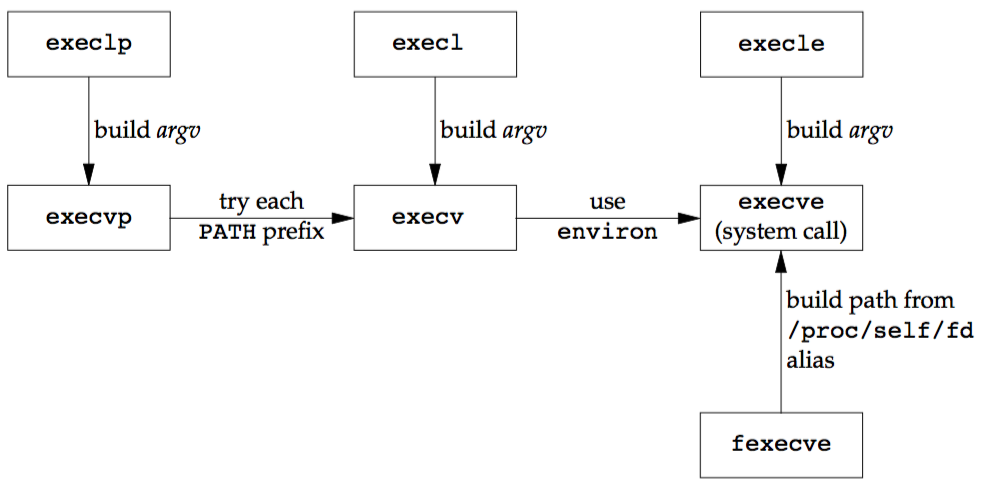
\includegraphics[width=0.9\linewidth]{figure/fig8-15_relationship.png}
    \caption{Relationship of the seven \texttt{exec} functions}
    \label{fig:relexec}
  \end{figure}
\end{frame}

\begin{frame}[containsverbatim,t]
  \frametitle{Example of \texttt{exec} Family}
\texttt{make echoall; ./echoall}

\lstinputlisting[linerange={7-14}, lineskip={0pt}]{codes/echoall.c}

\end{frame}


\begin{frame}[containsverbatim,t]
  \frametitle{Example of \texttt{exec} Family cont'd}
\texttt{make exec; ./exec}

\lstinputlisting[linerange={14-32}, lineskip={0pt}]{codes/exec.c}

\end{frame}



\section{Properties of Process}

\begin{frame}[t]
  \frametitle{Changing User IDs and Group IDs}
In the \textsc{Unix} system, privileges are based on user and group IDs
\begin{itemize}
\item change the system's current date
\item read or write a particular file
\end{itemize}

If a program can't access some resources, they need to change their user or group ID to gain appropriate privilege or access
\begin{itemize}
\item In general, we try to use the \textit{least-privilege} model
\item This reduces the risk that security might be compromised
\end{itemize}
\end{frame}

\begin{frame}[containsverbatim,t]
  \frametitle{APIs to Change User IDs and Group IDs}

\begin{codedef}
#include <unistd.h>
int setuid(uid_t uid);  // set the real and effective user ID
int setgid(gid_t gid);  // set the real and effective group ID
// Both return: 0 if OK, -1 on error
\end{codedef}

The rules for who can change the IDs (same applies to user ID and Group ID)
\begin{enumerate}
\item If the process has superuser privileges, the \texttt{setuid}
  function sets the real user ID, effective user ID, and saved
  set-user-ID to \textit{uid}.
\item If the process does not have superuser privileges, but
  \textit{uid} equals either the real user ID or the saved
  set-user-ID, \texttt{setuid} sets only the effective user ID to
  \textit{uid}. The real user ID and the saved set-user-ID are not
  changed.
\item If neither of these two conditions is true, \texttt{errno} is
  set to \texttt{EPERM} and \texttt{-1} is returned
\end{enumerate}

\end{frame}

\begin{frame}[t]
  \frametitle{Statements about the three user IDs}
  \begin{enumerate}
  \item \textbf{Only a superuser process can change the real user
    ID}. Normally, the real user ID is set by the \texttt{login(1)}
    program when we log in and never changes. Because login is a
    superuser process, it sets all three user IDs when it calls
    \texttt{setuid}.
  \item \textbf{The effective user ID is set by the \texttt{exec}
      functions only if the set-user-ID bit is set for the program
      file}. If the set-user-ID bit is not set, the \texttt{exec}
    functions leave the effective user ID as its current value. We can
    call \texttt{setuid} at any time to set the effective user ID to
    either the real user ID or the saved set-user-ID. Naturally, we
    can’t set the effective user ID to any random value.
  \item \textbf{The saved set-user-ID is copied from the effective
      user ID by exec}. If the file’s set-user-ID bit is set, this
    copy is saved after exec stores the effective user ID from the
    file’s user ID.
  \end{enumerate}
\end{frame}



\begin{frame}[t]
  \frametitle{Summary of setting the user IDs}
  \begin{figure}[h]
    \centering
    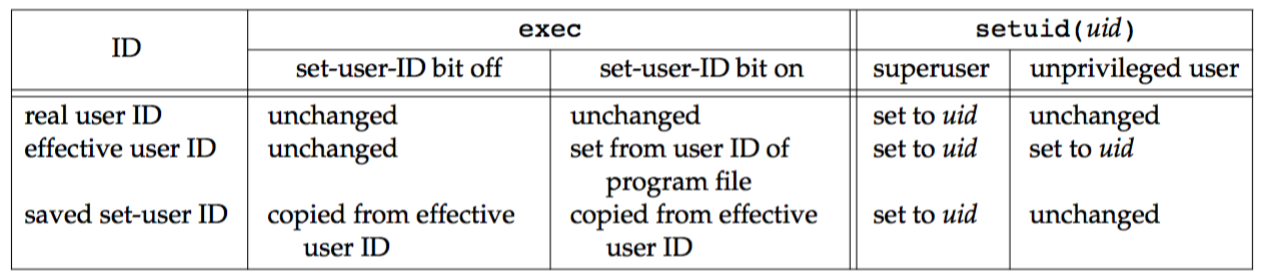
\includegraphics[width=\linewidth]{figure/fig8-18_ways.png}
    \caption{Ways to change the three user IDs}
    \label{fig:ways}
  \end{figure}
\end{frame}


\begin{frame}[containsverbatim,t]
  \frametitle{\texttt{setreuid} and \texttt{setregid} Functions}
BSD supported the swapping of the real user ID and the effective user ID
with the \texttt{setreuid} function.
\begin{itemize}
\item We can supply a value of -1 for any of the arguments to indicate that the corresponding ID should remain unchanged
\end{itemize}
\begin{codedef}
#include <unistd.h>
int setreuid(uid_t ruid, uid_t euid);
int setregid(gid_t rgid, gid_t egid);
// Both return: 0 if OK, -1 on error
\end{codedef}

The rule
\begin{itemize}
\item an unprivileged user can always swap between the real user ID and the effective user ID
\end{itemize}
\end{frame}


\begin{frame}[containsverbatim,t]
  \frametitle{\texttt{seteuid} and \texttt{setegid} Functions}
POSIX.1 includes the two functions \texttt{seteuid} and \texttt{setegid}. These functions are similar to \texttt{setuid} and \texttt{setgid}, but only the effective user ID or effective group ID is changed.
\begin{codedef}
#include <unistd.h>
int seteuid(uid_t uid);
int setegid(gid_t gid);
// Both return: 0 if OK, -1 on error
\end{codedef}
\end{frame}

\begin{frame}
  \frametitle{Summary of all functions}
  \begin{figure}[h]
    \centering
    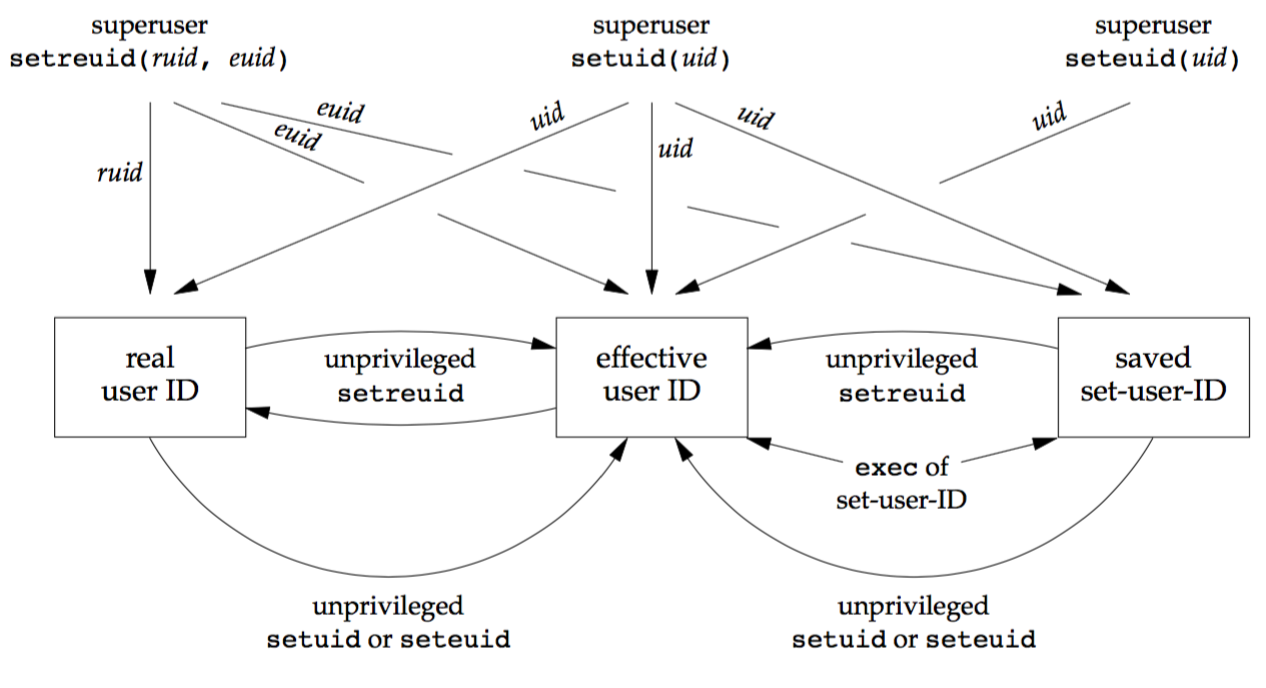
\includegraphics[width=\linewidth]{figure/fig8-19_summary.png}
    \caption{Summary of all the functions that set the various user IDs}
    \label{fig:summary}
  \end{figure}
\end{frame}







\section{Interpreter files and the \texttt{system} function}
\begin{frame}[t]
  \frametitle{Interpreter Files}
All contemporary UNIX systems support interpreter files. These files are text files that begin with a line of the form

\texttt{\#! pathname [ optional-argument ]}

The most common of these interpreter files begin with the line

\texttt{\#!/bin/sh}

\end{frame}

\begin{frame}[containsverbatim,t]
  \frametitle{Interpreter Files Example}

Example \textit{sharpbang} file
\lstinputlisting[lineskip=0pt]{codes/testinterp}

You have to change the PATHNAME on the interpreter line

Example \texttt{echoarg} program
\lstinputlisting[linerange={7-10}, lineskip=0pt]{codes/echoarg.c}
\end{frame}


\begin{frame}[containsverbatim,t]
  \frametitle{Interpreter Files Example}

Example interpreter files
\lstinputlisting[linerange={10-20},lineskip=0pt]{codes/interp.c}

You have to change the PWD in the code

{\footnotesize Note that on FreeBSD 8.0, \textit{pathname} limit is 4,097 bytes. On Linux 3.2.0, the limit is 128 bytes. Mac OS X 10.6.8 supports a limit of 513 bytes, whereas Solaris 10 places the limit at 1,024 bytes.}

\end{frame}



\begin{frame}[containsverbatim,t]
  \frametitle{\texttt{system} Function}
It is convenient to execute a command string from within a program

\texttt{system(``date > file'');}  is much simpler than to call \texttt{time} to get the current calendar time, then call \texttt{localtime} to convert it to a broken-down time, then call \texttt{strftime} to format the result

\begin{codedef}
#include <stdlib.h>
int system(const char *cmdstring);
// Returns: ---
\end{codedef}

\begin{enumerate}
\item If either the \texttt{fork} fails or \texttt{waitpid} returns an
  error other than \texttt{EINTR}, system returns \textbf{-1} with
  \texttt{errno} set to indicate the error.
\item If the \texttt{exec} fails, implying that the shell can’t be
  executed, the return value is as if the shell had executed
  \texttt{exit(127)}.
\item Otherwise, all three functions---\texttt{fork}, \texttt{exec},
  and \texttt{waitpid}---succeed, and the return value from system is
  the termination status of the shell, in the format specified for
  \texttt{waitpid}.
\end{enumerate}
\end{frame}

\begin{frame}[containsverbatim,t]
  \frametitle{The \texttt{system} Function Example}
read \texttt{codes/system.c}
\lstinputlisting[linerange={7-27},lineskip=0pt]{codes/system.c}
\end{frame}

\begin{frame}[containsverbatim,t]
  \frametitle{The \texttt{system} Function Example}
Run it with \texttt{make system; ./system}
\lstinputlisting[linerange={50-69},lineskip=0pt]{codes/system.c}
\end{frame}

\begin{frame}
  \frametitle{Security hole in using \texttt{system}}
\texttt{make tsys; make pruid}

\texttt{./tsys ./pruid}

\texttt{sudo chown root tsys ; chmod u+s tsys; ls -l tsys}

\texttt{./tsys ./pruid}

\lstinputlisting[linerange={22-31},lineskip=0pt]{codes/tsys.c}
\vspace{-0.8em}
\lstinputlisting[linerange={8-9},lineskip=0pt]{codes/pruid.c}

{\footnotesize Some implementations have closed this security hole by changing /bin/sh to reset the effective user ID to the real user ID when they don’t match. }
\end{frame}


\section{Miscellaneous}


\begin{frame}[containsverbatim,t]
  \frametitle{User Identification}
Any process can find out its real and effective user ID and group ID
\begin{itemize}
\item \texttt{getpwuid(getuid())} to find out the login name of the user who's running the program
\item If a single user has multiple login names, each with the same user ID, then we used \texttt{char *getlogin(void)} to find the login name
  \begin{itemize}
  \item \footnotesize A person might have multiple entries in the password file with the same user ID to have a different login shell for each entry
  \end{itemize}
\end{itemize}
\begin{codedef}
#include <unistd.h>
char *getlogin(void);
// Returns: pointer to string giving login name if OK, NULL on error
\end{codedef}
\end{frame}

\begin{frame}[containsverbatim,t]
  \frametitle{Process Scheduling}
A process can retrieve and change \textit{its} nice value with \texttt{nice} function
\begin{codedef}
#include <unistd.h>
int nice(int incr);
// Returns: new nice value - NZERO if OK, -1 on error

#include <sys/resource.h>
int getpriority(int which, id_t who);
// Returns: nice value between -NZERO and NZERO-1 if OK, -1 on error
int setpriority(int which, id_t who, int value);
// Returns: 0 if OK, -1 on error
\end{codedef}

\texttt{getpriority} function gets the \texttt{nice} value for a process
\begin{itemize}
\item \textit{which}: \texttt{PRIO\_PROCESS} to indicate a process,
  \texttt{PRIO\_PGRP} to indicate process group, and
  \texttt{PRIO\_USER} to indicate user ID
\item \textit{who}:  \texttt{0} indicates the calling process, process group, or user
  \begin{itemize}
  \item \footnotesize For example, when which is set to
    \texttt{PRIO\_USER} and \textit{who} is \texttt{0}, the real user
    ID of the calling process is used
  \end{itemize}

\end{itemize}
\end{frame}

\begin{frame}[containsverbatim,t]
  \frametitle{\texttt{nice} Example}
read \texttt{codes/nice.c}
\lstinputlisting[linerange={50-71},lineskip=0pt]{codes/nice.c}
\end{frame}

\begin{frame}[fragile,t]
  \frametitle{\texttt{nice} Example}

\texttt{make nice}

\begin{verbatim}
James@maker:codes$ ./nice
NZERO = 20
current nice value in parent is 20
current nice value in child is 20, adjusting by 0
now child nice value is 20
child count = 218686919
parent count = 218744258
James@maker:codes$ ./nice 20
NZERO = 20
current nice value in parent is 20
current nice value in child is 20, adjusting by 20
now child nice value is 39
parent count = 219145730
child count = 216745892
\end{verbatim}
\end{frame}


\begin{frame}[fragile,containsverbatim,t]
  \frametitle{Process Times}

There are three times that we can measure
\begin{enumerate}
\item \footnotesize wall clock time
\item \footnotesize user CPU time
\item \footnotesize system CPU time
\end{enumerate}

\begin{codedef}
#include <sys/times.h>
clock\_t times(struct tms *buf);
// Returns: elapsed wall clock time in clock ticks if OK, -1 on error
\end{codedef}

\begin{verbatim}
struct tms {
  clock_t  tms_utime;  /* user CPU time */
  clock_t  tms_stime;  /* system CPU time */
  clock_t  tms_cutime; /* user CPU time, terminated children */
  clock_t  tms_cstime; /* system CPU time, terminated children */
};
\end{verbatim}


\end{frame}


\begin{frame}[fragile,allowframebreaks,containsverbatim,t]
  \frametitle{Process Times Example }
\lstinputlisting[lineskip=0pt]{codes/times.c}

\end{frame}

\begin{frame}[fragile,t]
  \frametitle{Process Times Example}

\lstset{basicstyle=\footnotesize, numbers=none, lineskip=0pt}
\texttt{make times}

\texttt{./times "sleep 5" "date" "man bash > /dev/null"}
\vspace{-2em}
\begin{columns}[t]
  \begin{column}{0.45\linewidth}
\begin{lstlisting}
command: sleep 5
  real:     5.01
  user:     0.00
  sys:      0.00
  child user:     0.00
  child sys:      0.00
normal termination, exit status = 0

command: date
Mon Oct 10 14:26:00 KST 2016
  real:     0.01
  user:     0.00
  sys:      0.00
  child user:     0.00
  child sys:      0.00
normal termination, exit status = 0
\end{lstlisting}
  \end{column}
  \begin{column}{0.45\linewidth}
\begin{lstlisting}
command: man bash > /dev/null
  real:     0.29
  user:     0.00
  sys:      0.00
  child user:     0.29
  child sys:      0.08
normal termination, exit status = 0
\end{lstlisting}
  \end{column}
\end{columns}

\end{frame}


%---------------------------------------------------------
\section{Last Words}

\begin{frame}[t]
  \frametitle{Last Words}
\begin{itemize}
\item Read chapter 9
\item Read and run \texttt{./codes/master\_fork.c}
\item There are total of 18 examples.
\item Describe and explain the result for each \texttt{fork}s
\item Draw a diagram where possible, it helps you understanding the behavior
%\item Due date Oct-26
\end{itemize}
\end{frame}


\end{document}
